\documentclass[10pt,twocolumn]{article}

\usepackage[T1]{fontenc}
\usepackage[utf8]{inputenc}
\usepackage{newtxtext,newtxmath}
\usepackage[margin=0.72in,columnsep=0.25in]{geometry}
\usepackage{microtype}
\usepackage{amsmath}
\usepackage{booktabs}
\usepackage{array}
\usepackage{tabularx}
\usepackage{multirow}
\usepackage{graphicx}
\usepackage{xcolor}
\usepackage{enumitem}
\usepackage{caption}
\usepackage{subcaption}
\usepackage{natbib}
\usepackage{xurl}
\usepackage{hyperref}
\usepackage{tikz}
\usetikzlibrary{arrows.meta,positioning,shapes.geometric,fit}

\definecolor{graphblue}{HTML}{24557A}
\definecolor{entitygreen}{HTML}{4A7C59}
\definecolor{memorygray}{HTML}{5D6670}
\definecolor{lightblue}{HTML}{EAF2F8}
\definecolor{lightgreen}{HTML}{EDF5EF}
\definecolor{lightgray}{HTML}{F1F3F5}

\hypersetup{
  colorlinks=true,
  linkcolor=graphblue,
  citecolor=entitygreen,
  urlcolor=graphblue,
  pdfauthor={Shumao Sun},
  pdftitle={Entity-Memory Graph Retrieval Improves Evidence Coverage in Long-Conversation Question Answering}
}

\captionsetup{font=small,labelfont=bf}
\setlist{nosep,leftmargin=*}
\setlength{\parindent}{1em}
\setlength{\parskip}{0pt}
\setlength{\tabcolsep}{4pt}
\renewcommand{\arraystretch}{1.08}

\newcommand{\recallacc}{\texttt{recall\_acc}}
\newcommand{\bembed}{B_{\mathrm{embed}}}
\newcommand{\topk}{\textit{top-k}}

\title{\textbf{Entity--Memory Graph Retrieval Improves Evidence Coverage\\
in Long-Conversation Question Answering}}
\author{Shumao Sun\\
\small Affiliation to be supplied}
\date{}

\begin{document}
\maketitle

\begin{abstract}
Long-term conversational question answering requires a memory system to find
relevant evidence across temporally separated dialogue turns. We test whether
a conversation-built Entity--Memory graph improves retrieval over a matched
dense Memory control when Memory representations, query vectors, answer
generation, and evaluation are held fixed. Experiments cover 1,986
question--answer rows from ten LoCoMo conversations. At the primary cutoff
\topk{} 25, graph retrieval increases official evidence recall from 79.7468\%
to 84.4842\%. The 4.7374-point difference has paired-question and
conversation-cluster 95\% bootstrap intervals of 3.6504--5.8425 and
3.5286--6.0124 points. The recall advantage is supported at every
preregistered cutoff from 5 to 50, whereas no matched cutoff establishes an
overall final-answer F1 difference. Ablations associate the recall gain with
semantic scoring, Entity fusion, chronological expansion, and speaker links.
A complete cold/warm measurement records construction, indexing, retrieval,
provider usage, and storage. Warm retrieval averages 0.004886 seconds per
question after all cache-sensitive stages fall to zero new provider requests,
compared with 1.5123 seconds in the cold pass. The evidence supports a scoped
retrieval claim on the evaluated LoCoMo set. It does not establish improved
answer F1, cross-dataset generalization, official-reference parity, or
state-of-the-art performance.
\end{abstract}

\noindent\textbf{Keywords:} long-term conversational memory; graph retrieval;
evidence recall; retrieval-augmented generation; ablation analysis

\section{Introduction}

Conversational agents accumulate facts, events, preferences, and relationships
over interactions that exceed a model's usable context. Long-term memory
systems must therefore decide what to store, how to organize it, and which
parts to retrieve for a new question. The LoCoMo benchmark makes this problem
concrete through long, multi-session conversations and questions requiring
single-hop, multi-hop, temporal, commonsense, and adversarial reasoning
\citep{maharana2024locomo}. Long-context and retrieval-augmented generation
improve memory-related question answering on LoCoMo, but long-range temporal
and causal reasoning remain difficult.

Dense retrieval provides a natural control. It encodes each conversational
Memory item, scores that item against the question, and sends the
highest-ranked items to an answer model. The design is simple and scalable,
but it treats Memory items as independent. A graph can represent repeated
entities and chronological adjacency, allowing retrieval to use structure
that is absent from a flat index. A valid comparison must distinguish that
structural contribution from changes in embeddings, context budgets, answer
models, or evaluation.

We evaluate an Entity--Memory graph built only from conversation content.
Each dialogue item becomes a Memory node, normalized Entities become shared
nodes, and chronological links connect neighboring Memories. Entity matching
is fused with semantic Memory similarity and chronological expansion at query
time. Test questions form retrieval queries only. Questions, answers, evidence
labels, categories, predictions, and evaluator output are excluded from graph
construction.

This study asks three questions. First, does the graph improve evidence recall
over matched dense retrieval when Memory vectors, query vectors, answer
generation, and evaluation are fixed? Second, which graph components are
associated with any observed difference? Third, does the result persist across
retrieval cutoffs and selected input, fusion-weight, and sequence-scale
settings? The experiments address these questions through:

\begin{enumerate}[label=(\arabic*)]
  \item an all-question matched comparison with immutable ordered query
  vectors and identical answer generation;
  \item separate measurement of evidence recall and final-answer F1 with
  paired-question and conversation-cluster uncertainty; and
  \item component, input, cutoff, parameter, and cold/warm system analyses
  under frozen protocols.
\end{enumerate}

The result is narrower than a general memory-system claim. Complete graph
retrieval improves evidence recall across \topk{} 5, 10, 25, and 50 on the
evaluated ten-conversation set, but it does not establish higher overall
answer F1.

\section{Related Work}

\subsection{Retrieval foundations and long-context organization}

Retrieval-augmented generation combines a parametric generator with retrieved
non-parametric evidence \citep{lewis2020rag}. Dense Passage Retrieval showed
that a learned dual encoder can retrieve candidate passages for open-domain
question answering using dense representations
\citep{karpukhin2020dpr}. These studies establish the flat dense-retrieval
control used in our matched comparison.

Later systems organize long inputs above the individual-chunk level. RAPTOR
recursively embeds, clusters, and summarizes text into a retrieval tree
\citep{sarthi2024raptor}. MemoRAG uses a long-range model to form global memory
and generate clues for a downstream retriever \citep{qian2024memorag}. Our
method also introduces structure above independent Memory vectors, but it
retains dialogue items as the answer evidence rather than replacing them with
generated summaries.

\subsection{Long-term conversational memory}

LoCoMo introduced a human-verified benchmark of long, persona-grounded,
multimodal conversations and evaluates question answering, event
summarization, and dialogue generation \citep{maharana2024locomo}.
LongMemEval later framed assistant memory as indexing, retrieval, and reading,
and evaluates information extraction, multi-session reasoning, temporal
reasoning, knowledge updates, and abstention \citep{wu2025longmemeval}. These
benchmarks motivate pipeline-level evaluation rather than attributing all
downstream behavior to the language model.

Early agent-memory architectures store experience for later retrieval and
reflection. Generative Agents records observations, derives higher-level
reflections, and retrieves memories for planning
\citep{park2023generative}. MemoryBank adds persistent conversational memory
with retrieval, updating, and time-dependent forgetting
\citep{zhong2024memorybank}. MemGPT instead manages limited context through
virtual memory and hierarchical tiers \citep{packer2023memgpt}.

Recent systems place more structure in the memory store. Mem0 extracts,
consolidates, and retrieves salient conversational information, with a graph
variant for relational memory \citep{chhikara2025mem0}. A-Mem dynamically
indexes and links structured memory notes into an evolving network
\citep{xu2025amem}. Our study examines a narrower question than these
end-to-end memory architectures. Given a fixed reader and fixed Memory
representations, we test whether a conversation-derived graph changes evidence
retrieval relative to a flat dense control.

\subsection{Graph retrieval}

Graph retrieval can expose relations that independent text chunks omit.
HippoRAG combines a knowledge graph with Personalized PageRank for long-term
knowledge integration and multi-hop retrieval
\citep{gutierrez2024hipporag}. GraphRAG constructs a graph index and community
summaries for global questions over document collections
\citep{edge2024graphrag}. GRAG retrieves textual subgraphs and supplies textual
and topological views to a generator \citep{hu2025grag}, while LightRAG
combines graph indexing with dual-level retrieval over entities and relations
\citep{guo2025lightrag}.

Graph structure has also become central to conversational memory. APEX-MEM
stores temporally grounded events in a property graph and resolves evolving
information at retrieval time \citep{banerjee2026apexmem}. Mnemis combines a
base similarity graph with top-down selection over a semantic hierarchy
\citep{tang2026mnemis}. GAM separates an event-progression graph from a
topic-association network \citep{wu2026gam}, whereas TiMem consolidates
conversation observations into a temporal hierarchy
\citep{li2026timem}. Our graph is smaller in scope. Shared Entity nodes link
mentions across dialogue-item Memories, and chronological edges preserve local
sequence. The methodological emphasis is a matched retrieval control and the
separation of evidence recall from generated-answer F1.

\subsection{Dense retrieval controls}

DRAGON is a dense retriever trained with diverse data augmentation
\citep{lin2023dragon} and is used in the original LoCoMo RAG setup. We
inspected the pinned upstream reference but did not pass the project's official
reproduction tolerance. A local raw-DRAGON condition is therefore retained
only as a diagnostic. It is excluded from controlled and inferential claims.
The formal comparison in this paper is internal and matched. Dense Memory
retrieval is compared with graph retrieval using identical Memory and query
vector artifacts.

\section{Method}

\begin{figure*}[t]
\centering
\resizebox{\textwidth}{!}{%
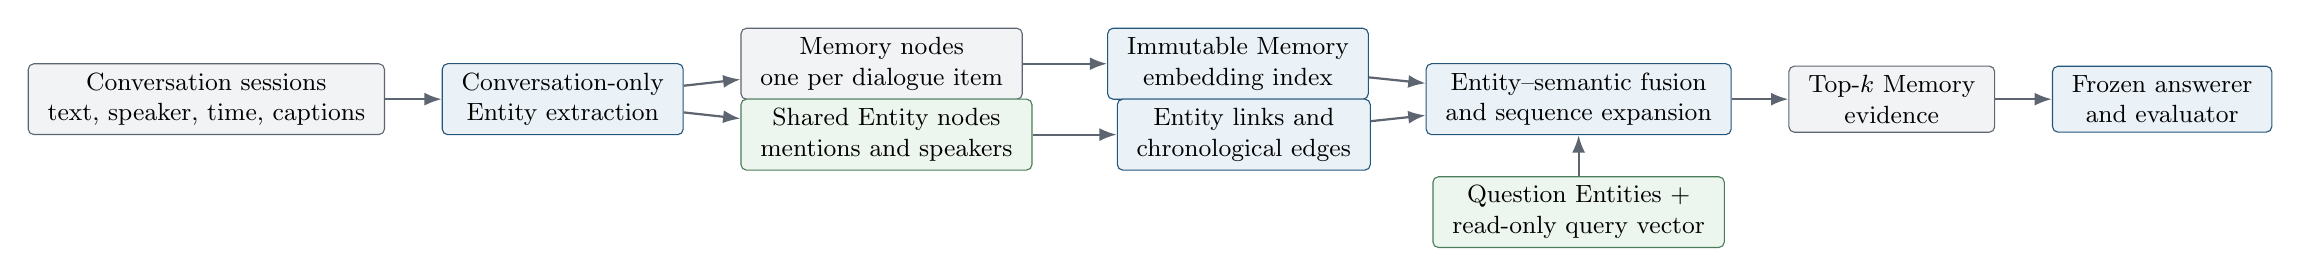
\begin{tikzpicture}[
  node distance=0.65cm and 0.72cm,
  box/.style={draw,rounded corners=2pt,minimum height=0.72cm,
    align=center,font=\small,inner xsep=7pt},
  memory/.style={box,fill=lightgray,draw=memorygray},
  entity/.style={box,fill=lightgreen,draw=entitygreen},
  process/.style={box,fill=lightblue,draw=graphblue},
  arrow/.style={-{Latex[length=2.2mm]},thick,draw=memorygray}
]
\node[memory] (conv) {Conversation sessions\\text, speaker, time, captions};
\node[process,right=of conv] (extract) {Conversation-only\\Entity extraction};
\node[memory,right=of extract,yshift=0.45cm] (mem) {Memory nodes\\one per dialogue item};
\node[entity,right=of extract,yshift=-0.45cm] (ent) {Shared Entity nodes\\mentions and speakers};
\node[process,right=of mem,xshift=0.35cm] (index) {Immutable Memory\\embedding index};
\node[process,right=of ent,xshift=0.35cm] (graph) {Entity links and\\chronological edges};
\node[process,right=of index,yshift=-0.45cm] (fusion) {Entity--semantic fusion\\and sequence expansion};
\node[memory,right=of fusion] (context) {Top-\(k\) Memory\\evidence};
\node[process,right=of context] (reader) {Frozen answerer\\and evaluator};
\node[entity,below=0.52cm of fusion] (query) {Question Entities +\\read-only query vector};

\draw[arrow] (conv) -- (extract);
\draw[arrow] (extract) -- (mem);
\draw[arrow] (extract) -- (ent);
\draw[arrow] (mem) -- (index);
\draw[arrow] (ent) -- (graph);
\draw[arrow] (index) -- (fusion);
\draw[arrow] (graph) -- (fusion);
\draw[arrow] (query) -- (fusion);
\draw[arrow] (fusion) -- (context);
\draw[arrow] (context) -- (reader);
\end{tikzpicture}%
}
\caption{The experimental retrieval path. Graph construction consumes only
conversation fields. Questions enter after construction through a
question-Entity extractor and a read-only query-vector artifact. The matched
dense control uses the same Memory nodes, Memory vectors, query vectors,
answerer, and evaluator, but omits Entity fusion and sequence expansion.}
\label{fig:pipeline}
\end{figure*}

\subsection{Conversation-only graph construction}

Figure~\ref{fig:pipeline} summarizes the experimental path. For each
conversation, the constructor consumes session timestamps, dialogue
identifiers, speaker names, dialogue text, and image captions. Each normalized
dialogue item becomes a Memory node. A \texttt{gpt-3.5-turbo} extractor at
temperature 0.3 identifies Entities from the conversation text. Entity strings
are normalized, deduplicated case-insensitively, and connected to every Memory
in which they occur. Deterministic speaker links add the dialogue speaker as an
Entity. Adjacent Memory nodes are connected in chronological order.

The complete ten-conversation graph contains 5,882 Memory nodes. Graph
construction does not consume QA questions, gold answers, evidence
annotations, category labels, judge outputs, previous predictions, or
question-driven ledgers. This separation prevents test questions from shaping
the stored memory structure.

\subsection{Retrieval}

The question supplies two retrieval-only signals. A question-Entity extractor
first produces normalized keys for matching Entity nodes. The question then
retrieves its vector from a complete, immutable
\texttt{text-embedding-3-small} artifact. The artifact is bound to the dataset
hash, ordered question digests, model, role, vector dimension, normalization,
and artifact SHA-256. Formal retrieval fails on a cache miss and makes no live
query-embedding request.

For Memory \(m\), the primary condition combines Entity relevance \(s_e(m)\)
and signed semantic similarity \(s_s(m)\):
\begin{equation}
s(m)=0.30s_e(m)+0.70s_s(m).
\label{eq:fusion}
\end{equation}
Entity candidates must reach a relative-score threshold of 0.5, with at most
20 matches retained per query key. Speaker-only matches are multiplied by
0.25, and Entity contributions are degree-discounted. Chronological neighbors
are expanded at secondary scale 0.5. If the gated pool contains fewer than the
requested number of Memories, semantic full-pool retrieval fills the remaining
positions without discarding gated results. Candidates are ordered by
descending fused score and then dialogue id.

The primary context budget is \topk{} 25. Cutoff analyses use \topk{} 5, 10,
and 50. The dense control ranks the same Memory representations with the same
semantic query vectors but does not use Entity matching or sequence expansion.
A dense graph-construction control, \(\bembed\), verifies that graph
construction alone does not change dense retrieval.

\subsection{Answer generation and evaluation}

Retrieved Memory text and identifiers enter the frozen LoCoMo-aligned answer
interface. The requested answer model is \texttt{gpt-3.5-turbo}, with a
system-role prompt, temperature 0, one question per batch, and a 32-token
completion limit. The immutable evaluation package retains its
category-specific generation, decoding, F1, evidence-recall, rounding, and
aggregation behavior.

We report two outcomes. Overall F1 measures final-answer overlap under the
frozen evaluator. \recallacc{} is the official evidence-recall definition.
The repository-defined Categories 1--4 subset F1 is used only as a diagnostic
and is not presented as an official LoCoMo metric.

\subsection{Statistical analysis}

Every formal condition contains the same 1,986 QA rows from ten conversations.
Matched differences are estimated with 10,000 paired-question bootstrap
resamples and 10,000 resamples of whole conversations, using seed 20260727.
The conversation-cluster estimator reflects uncertainty over the ten
conversation units. Component, input, fusion, and sequence families use Holm
step-down correction within each outcome and estimator. A difference is
treated as supported only when the preregistered evidence gate passes. Failure
to reject is not interpreted as equivalence.

\section{Experimental Design}

The primary comparison holds constant the dataset and row order, Memory text,
Memory vectors, immutable ordered query vectors, answer prompt, answer model,
token budget, evaluation package, output isolation, and aggregation. The
treatment activates Entity matching, graph fusion, and chronological
expansion. The \(\bembed\) control must reproduce the dense control's ordered
context identifiers for all rows before the primary graph contrast is
interpreted.

Component conditions remove sequence expansion, Entity-score fusion, or the
semantic channel. A speaker ablation removes deterministic speaker links.
Input conditions compare time-annotated and raw-text profiles. Sensitivity
families vary Entity/Semantic weights and chronological scale. Cutoff analysis
uses matched A/B pairs at \topk{} 5, 10, 25, and 50.

Each metric-bearing condition writes to an absent, condition-specific output
directory. The record includes the source commit, resolved configuration,
model names, artifact identities, query-cache hits and misses, prompt budgets,
and graph compliance. The vendored evaluator is verified against its SHA-256
manifest before formal use.

\section{Results}

\subsection{Primary matched comparison}

\begin{table}[t]
\centering
\caption{Primary matched comparison at \topk{} 25. Values are percentages.}
\label{tab:primary}
\begin{tabular}{@{}lrr@{}}
\toprule
Condition & Overall F1 & \recallacc{} \\
\midrule
A (dense Memory) & 42.0681 & 79.7468 \\
\(\bembed\) (dense graph control) & 42.0677 & 79.7468 \\
B (complete graph retrieval) & \textbf{42.5680} & \textbf{84.4842} \\
\bottomrule
\end{tabular}
\end{table}

Complete graph retrieval improves \recallacc{} over the matched dense control
by 4.7374 percentage points (Table~\ref{tab:primary}). The paired-question
95\% interval is 3.6504--5.8425 points, and the conversation-cluster interval
is 3.5286--6.0124 points. Both two-sided \(p\)-values are 0.0002. Overall F1
changes by 0.4998 points, with paired and cluster intervals of
\(-0.5745\)--1.5514 and \(-0.1773\)--1.2711 points. The F1 difference is not
supported by either estimator.

The dense graph-construction control and A have zero ordered-context
mismatches across all 1,986 rows and identical evidence recall. Their F1
values differ by less than 0.001 percentage points, consistent with frozen
Category-5 option-order randomness rather than a retrieval difference.

\subsection{Cutoff analysis}

\begin{table*}[t]
\centering
\caption{Matched cutoff analysis. Values are percentages; differences are
B minus A in percentage points. Every paired-question and
conversation-cluster recall interval is above zero. Every corresponding F1
interval includes zero.}
\label{tab:cutoffs}
\begin{tabular}{@{}rrrrrrrll@{}}
\toprule
\topk{} & A F1 & B F1 & \(\Delta\)F1 & A recall & B recall &
\(\Delta\)recall & Paired recall CI & Cluster recall CI \\
\midrule
5  & 39.9053 & 39.8264 & \(-0.0790\) & 59.3584 & 64.1667 & \(+4.8083\) & [3.3450, 6.2808] & [2.8809, 6.6134] \\
10 & 41.7607 & 42.1412 & \(+0.3805\) & 68.9145 & 74.4847 & \(+5.5702\) & [4.2928, 6.8624] & [4.2365, 6.7522] \\
25 & 42.0681 & 42.5680 & \(+0.4998\) & 79.7468 & 84.4842 & \(+4.7374\) & [3.6504, 5.8425] & [3.5286, 6.0124] \\
50 & 42.0782 & 41.7832 & \(-0.2950\) & 86.7148 & 90.3306 & \(+3.6159\) & [2.7754, 4.4735] & [2.4603, 4.6426] \\
\bottomrule
\end{tabular}
\end{table*}

The evidence-recall advantage persists across all preregistered cutoffs
(Table~\ref{tab:cutoffs}). B minus A recall differences range from 3.6159 to
5.5702 points. Paired-question and conversation-cluster intervals are above
zero at every cutoff. Both matched F1 intervals include zero at every cutoff.
The cutoff analysis therefore supports an evidence-coverage advantage over the
tested range, not an answer-quality advantage.

\subsection{Components, inputs, and sensitivity}

\begin{table*}[t]
\centering
\caption{Component and input contrasts at \topk{} 25. Differences are
treatment minus control in percentage points. ``Supported'' refers to the
preregistered family-corrected inference unless noted otherwise.}
\label{tab:components}
\begin{tabularx}{\textwidth}{@{}Xrrl@{}}
\toprule
Contrast & \(\Delta\)F1 & \(\Delta\)\recallacc{} & Conclusion \\
\midrule
B minus B without sequence expansion & \(+0.5137\) & \(+1.6728\) & Recall supported; F1 not supported \\
B minus B without Entity-score fusion & \(+0.8014\) & \(+4.7626\) & Recall supported; F1 not supported \\
Sequence expansion after Entity gating & \(-0.0609\) & \(+0.4364\) & Recall supported; F1 not supported \\
B minus Entity-only retrieval & \(+5.0780\) & \(+17.4634\) & Both outcomes supported \\
Raw-text B minus annotated-input B & \(+0.2407\) & \(-0.2472\) & Neither outcome supported \\
Raw-text B minus raw-text A & \(+0.3508\) & \(+4.9522\) & Recall supported; F1 not supported \\
B minus B without speaker links & \(+0.2415\) & \(+1.4822\) & Recall supported; F1 not supported \\
\bottomrule
\end{tabularx}
\end{table*}

Several graph operations are associated with the retrieval gain
(Table~\ref{tab:components}). Complete B improves recall over the no-sequence
condition by 1.6728 points and over the no-Entity-score-fusion condition by
4.7626 points after Holm correction. Neither contrast supports F1. Sequence
expansion after Entity gating contributes 0.4364 recall points. The semantic
channel relative to Entity-only retrieval contributes 17.4634 recall points
and 5.0780 F1 points, with both outcomes supported within the component
family. Removing deterministic speaker links lowers recall by 1.4822 points
without a supported F1 change.

Input and parameter results bound these component findings. Time annotation
has no supported within-B overall effect after correction. When both A and B
use raw text, B retains a supported 4.9522-point recall advantage without an
F1 advantage. Reducing Entity/Semantic weights from 0.30/0.70 to 0.10/0.90
lowers recall by 2.3062 points after correction. Equal 0.50/0.50 weights are
not distinguishable from the primary setting. No overall F1 or recall
contrast among sequence scales 0.25, 0.5, and 1.0 survives family correction.

\subsection{Cold and warm system cost}

\begin{table*}[t]
\centering
\caption{Primary-B cold and warm system measurement. Stage wall times overlap
and must not be summed as end-to-end latency.}
\label{tab:cost}
\begin{tabularx}{\textwidth}{@{}>{\raggedright\arraybackslash}Xr
  >{\raggedright\arraybackslash}X
  >{\raggedright\arraybackslash}Xr
  >{\raggedright\arraybackslash}X@{}}
\toprule
Stage & Cold req. & Cold tokens (input/output) & Cold timing & Warm req. & Warm timing \\
\midrule
Conversation Entity extraction & 5,873 & 3,731,393 / 425,637 & 9,792.76 s summed call time & 0 & 0.00 s \\
Memory embedding & 591 & 214,229 / 0 & 443.38 s & 0 & 1.29 s cache load \\
Question Entity extraction & 1,974 & 1,214,259 / 104,272 & 2,970.83 s & 0 & 0.00 s \\
Retrieval (1,986 QA) & 0 & 0 / 0 & mean 1.5123 s; p95 2.6132 s & 0 & mean 0.004886 s; p95 0.006270 s \\
\bottomrule
\end{tabularx}
\end{table*}

The warm replay makes no new provider requests in the three cache-sensitive
stages (Table~\ref{tab:cost}). Mean retrieval latency is 309.48 times lower.
Cold and warm each cover the same 44 ordered batches, with 1,998 reads from the
immutable query artifact, zero misses, and zero live query embeddings. The
formal answer trace contains 1,986 requests, 2,744,099 input tokens, and
16,269 output tokens. Because answer generation is independent of cache
warmth, the same validated trace is attached to each state rather than rerun.

Graphs occupy 21,689,931 bytes, Memory indexes 29,946,660 bytes, and
Entity/question caches 3,411,176 bytes. Monetary cost is not reported because
provider pricing was not frozen as an experimental input.

\section{Discussion}

The experiments separate evidence coverage from answer quality. Entity links,
semantic scoring, and chronological expansion retrieve more annotated
evidence than the matched dense control, and the difference persists across
four context budgets. The fixed short-answer generator does not convert the
additional coverage into a supported overall F1 gain. Evaluations that report
only answer scores can therefore obscure retrieval changes, while retrieval
improvements should not be described as end-to-end quality gains.

This separation complements LongMemEval's decomposition of assistant memory
into indexing, retrieval, and reading stages \citep{wu2025longmemeval}.
Systems such as Mem0, A-Mem, APEX-MEM, Mnemis, GAM, and TiMem jointly change
several of these stages
\citep{chhikara2025mem0,xu2025amem,banerjee2026apexmem,tang2026mnemis,wu2026gam,li2026timem}.
Their published scores therefore answer broader system-level questions than
our matched contrast. Differences in readers, graph construction, prompts,
context budgets, and metrics preclude a numerical ranking against our result.
Our evidence instead identifies what changes when the stored Memory text,
Memory vectors, query vectors, answerer, and evaluator remain fixed.

The component results suggest that the complete difference is distributed
across the retrieval path. The semantic channel is the largest isolated
contributor. Entity fusion, sequence expansion, and speaker links add smaller
supported recall contributions. The raw-text comparison indicates that the
B-over-A recall advantage does not depend on the tested time annotation.
Sensitivity results also discourage presenting the primary parameters as
universally optimal. One lower-Entity-weight condition reduces recall, an
equal-weight condition is not distinguishable, and no tested sequence scale
survives family correction.

The cold/warm result exposes an operational tradeoff. Conversation Entity
extraction and Memory embedding are one-time costs, while uncached
question-Entity extraction dominates cold retrieval latency. Once the
conversation artifacts and question-Entity cache are present, the graph path
requires no new provider request before answer generation and retrieval takes
milliseconds per question. This result is relevant for repeated evaluation
and repeated queries, but it does not imply the same latency on another
machine, provider, or workload.

\subsection{Limitations and future work}

First, formal evidence comes from ten conversations in one LoCoMo release.
Conversation-cluster bootstrap reflects uncertainty over these ten units but
does not establish cross-dataset generalization. Replication on additional
conversation-memory benchmarks is needed.

Second, no matched cutoff supports an overall final-answer F1 difference. The
contribution concerns retrieval coverage, not a general improvement in
generated answers. Alternative readers and evidence selectors require
separately controlled experiments.

Third, the official DRAGON reproduction gate did not pass. The local raw
DRAGON experiment changes semantic and query artifacts and remains diagnostic.
A future official-reference comparison requires parity with the pinned
upstream implementation.

Fourth, the requested answer-model name is recorded, but the provider did not
persist a separate actual-model identity in the formal snapshots. Category 5
also retains the frozen upstream unseeded option-order behavior. Future runs
should preserve provider-returned model identities when available and quantify
Category-5 generation variance separately.

Finally, system timing was measured on one machine and one provider endpoint.
The warm condition assumes complete reusable graph, index, and
question-Entity artifacts. Replication across hardware and providers is
needed before deployment-level latency claims.

\section{Reproducibility and Responsible Use}

Every formal condition records its source commit, resolved configuration,
dataset and artifact SHA-256 values, isolated output path, query-cache usage,
provider-token telemetry, graph-input audit, and prompt budget. Query vectors
are complete and read-only during formal retrieval. The evaluation package is
vendored and hash-verified. Statistical reports and the final cost report have
independent byte-identical reproductions.

The graph uses conversation data, including speaker names and image captions,
which can contain personal information in real deployments. Systems applying
this method outside the benchmark should establish consent, retention,
deletion, and access-control policies. The present work evaluates benchmark
retrieval and does not study privacy attacks or sensitive-memory deletion.

\section{Conclusion}

Long-conversation question answering requires retrieval that preserves
relevant evidence without using test questions to build memory. Graph
retrieval may represent links that a flat index omits, but a fair test must
hold the dense representations, query vectors, answer generation, and
evaluation fixed. Our matched design addresses this evidence gap.

The Entity--Memory graph improves official evidence recall over dense Memory
retrieval across \topk{} 5--50 on the evaluated LoCoMo set. Component analyses
associate the recall difference with semantic scoring, Entity fusion,
chronological expansion, and speaker links. The same experiments do not
establish higher overall final-answer F1. Finally, the cold/warm measurement
shows that reusable graph, index, and question-Entity artifacts remove new
provider requests from the retrieval path before answer generation.

This work is best viewed as a scoped retrieval study. The ten-conversation
sample, failed official DRAGON reproduction gate, fixed reader, and
single-environment latency measurement bound the claim. Separating evidence
coverage from answer quality provides a transferable evaluation principle for
future long-term conversational memory systems.

\section*{Data and Code Availability}

LoCoMo data are available from the benchmark authors
\citep{maharana2024locomo}. Code, experiment manifests, validation records,
and manuscript evidence snapshots for this study are available at
\url{https://github.com/Sun668/graph_memory}. The exact manuscript snapshot
corresponds to the repository history recorded with the arXiv source bundle.

\section*{Acknowledgments}

Affiliation, acknowledgments, funding information, and contribution statements
will be added when supplied.

\bibliographystyle{plainnat}
\bibliography{references}

\appendix
\onecolumn

\section{Resolved Primary Configuration}
\label{app:config}

\begin{table}[h]
\centering
\caption{Resolved settings for the primary B condition.}
\label{tab:config}
\begin{tabular}{@{}ll@{}}
\toprule
Dimension & Resolved value \\
\midrule
Dataset & LoCoMo ten-conversation release; 1,986 QA rows \\
Graph inputs & Session time, dialogue id, speaker, text, image caption \\
Excluded graph inputs & Questions, answers, evidence, categories, judges, predictions \\
Memory nodes & 5,882 \\
Conversation Entity extractor & \texttt{gpt-3.5-turbo}; temperature 0.3 \\
Memory embedding model & \texttt{text-embedding-3-small} \\
Answer model request & \texttt{gpt-3.5-turbo}; temperature 0; 32 output tokens \\
Primary context budget & \topk{} 25 \\
Entity / semantic weights & 0.30 / 0.70 \\
Entity relative-score threshold & 0.5 \\
Maximum matches per Entity key & 20 \\
Speaker-only dampening & 0.25 \\
Degree discount & Enabled \\
Sequence expansion scale & 0.5 \\
Query embeddings & Complete read-only artifact; L2-normalized float32 \\
Bootstrap & 10,000 paired QA and 10,000 conversation-cluster resamples \\
Bootstrap seed & 20260727 \\
\bottomrule
\end{tabular}
\end{table}

\section{Validity and Reproducibility Gates}

\begin{table}[h]
\centering
\caption{Checks applied before promotion of formal evidence.}
\label{tab:gates}
\begin{tabularx}{\textwidth}{@{}lXl@{}}
\toprule
Gate & Requirement & Outcome \\
\midrule
Graph construction & Conversation-only inputs; no QA-derived construction fields & Pass \\
Evaluator integrity & All 16 vendored files match the frozen SHA-256 manifest & Pass \\
Output isolation & One absent or empty directory per resolved formal condition & Pass \\
Query vectors & Complete ordered coverage; zero miss; zero live query embedding & Pass \\
Dense control & A and \(\bembed\) ordered contexts equal for all 1,986 rows & Pass \\
Prompt budget & Non-data scaffold no longer than 5,000 characters & Pass (2,410) \\
Statistical reproduction & Independent report build is byte-identical & Pass \\
Cost reproduction & Independent cost report build is byte-identical & Pass \\
Cache preservation & Quarantined artifacts retain frozen identities & Pass \\
\bottomrule
\end{tabularx}
\end{table}

\section{Claim Boundary}

The strongest supported statement is that complete conversation-built
Entity--Memory retrieval improves official evidence recall over matched dense
Memory retrieval across \topk{} 5, 10, 25, and 50 on the evaluated
ten-conversation LoCoMo set. The evidence does not support an overall
final-answer F1 advantage, cross-dataset generalization, an official DRAGON
comparison, state-of-the-art status, or monetary cost. These exclusions apply
to the Abstract, Results, Discussion, and Conclusion.

\end{document}
